\documentclass[../../../main.tex]{subfiles}
\begin{document}

To simulate a solid using finite element analysis, it is necessary to have a volumetric mesh of that solid. 
Unlike surface meshes, volumetric meshes allow both the interior and the surface of the solid to be represented, as they are composed of three-dimensional elements. 
Without them, it is not possible to simulate the deformation of a solid. 

Therefore, the next step will be to obtain the volumetric mesh of the solid structure. 
To do this, the surface mesh of the solid must first be obtained, as it will be needed to fabricate the structure. 
Subsequently, the volumetric mesh will be obtained from the surface mesh. 
There is specialised software for generating meshes. 
However, this software requires the user to design the geometry manually. 
In this case, it is not feasible to generate the structure manually, so algorithms and meshing libraries were used to create both meshes. 
This chapter explains how both meshes were obtained.

\subsection{Mesh generation procedure }

There are various ways and algorithms for generating the surface mesh of a geometric domain. 
In the present case, the geometric domain will be the surface of the edges and the joints at the nodes. 
The edges can be modelled as cylinders and the nodes as spheres. 
This is the simplest method for generating a surface mesh for a reticular structure, and the first one used.
Spheres could even be avoided for the nodes if a more continuous structure is preferred. 
To generate the mesh in this way, the Python Trimesh\cite{trimesh} library was used. 
This library specialises in the generation of triangular meshes and contains routines for generating cylindrical and spherical meshes. 
A submodule was developed to generate the mesh of the structure generated by the generation routine, and it was included inside the workflow complete module. Since the developed algorithm that generates the structure stores it as a graph, by placing cylinders of the desired radius on each of the edges of the graph, the surface mesh of the entire structure can be obtained. 
Various optimisations were carried out to improve the efficiency of this submodule, and maximum efficiency was achieved by parallelising the creation of the surfaces. 
\cref{fig:mesh_1} shows an example of the mesh of a structure obtained from a cylinder with a diameter of 2 \textit{cm} and a height of 3 \textit{cm}. 
Cylinders with a diameter of 1 \textit{mm} were used to generate the mesh.

\begin{figure}[!htbp]
    \centering
    \includegraphics[width= 0.4\textwidth]{imgs/mesh_1.png}
    \caption{Example of the mesh of a structure obtained from a cylinder with a diameter of 2 \textit{cm} and a height of 3 \textit{cm}. Cylinders with a diameter of 1 \textit{mm} were used to generate the mesh. No spheres were used to recreate the nodes.}
    \label{fig:mesh_1}
\end{figure}

As mentioned above, this is the simplest solution and is only useful for printing the structure in 3D. 
However, this surface does not actually represent a continuous surface, as the elements are not joined together. 
All that has been done is to place cylinders at the positions of the edges, but at no point have they been joined to form a single surface. 
To do this, it is necessary to use Boolean mesh operations, which allow obtaining the union, difference and intersection between pairs of meshes. 
In this case, it is only necessary to use the union operation to obtain a single surface. 
The same library used to generate the mesh contains routines to perform these Boolean operations. However, it does not perform the operations natively but uses the Manifold3D\footnote{\href{https://pypi.org/project/manifold3d/}{Manifold3D}.} or Blender\cite{blender} library kernels to perform them. 
The cylinders were joined in stages by joining subsets of cylinders. 
The total number of cylinders is divided into a pre-established number of batches, and in batch of these groups the joining operations are carried out as follows: the first cylinder in the set is selected and merged with the second, the resulting surface from this join is joined with the third cylinder, and so on until the group is complete and a single surface is obtained. 
This is done in this way so that the process of joining the cylinders in each of the groups can be parallelised. 
Subsequently, all the groups are joined in the same way. 
If spheres are included in the nodes, they are joined one by one to the final single surface, as this process cannot be parallelised.

Virtually none of the cases processed were able to complete the joining of all surfaces due to the complex shape of the intersections of the cylinders at some nodes. 
Therefore, it was decided to rely on a more powerful computational geometry library. 
The Gmsh\cite{Geuzaine2009} library was used, which has a Python API that allows the vast majority of its routines to be used, as the native library is written in C++. 
In addition, this library allows certain routines from the OpenSCAD\footnote{\href{https://openscad.org/}{OpenSCAD} official website.} library to be used to perform some operations. 
Gmsh library uses different and robust algorithms than Manifold3D or Blender to resolve intersections in surface joints. 
It also allows for generating meshes, so the process of generating cylindrical surfaces was also transferred to that library. 
After many attempts to generate the surface mesh, it was not possible to generate the surface mesh using Gmsh. 
The intersections of the nodes are too complex even for the most robust algorithms. 
After Gmsh, the TetGen\cite{tetgen} library was used, but also without success. 
Boolean operations are complex and computationally expensive to perform, so Python libraries that work with meshes rely on libraries written in C++ to perform them. 
Although this same thing occurs within mesh libraries written in C++. 
Very few libraries natively implement mesh manipulation routines; almost all of them resort to existing libraries to perform any operation and offer certain improvements in the aspects for which those libraries were designed. 
The de facto standard for computational geometry is the CGAL\cite{cgal} (Computational Geometry Algorithms Library), written in C++. 
The vast majority of computational geometry libraries are based on this library. 
However, others are autonomous and also widely used, such as TetGen, Gmsh, and VCGlib\footnote{\href{http://vcglib.net/index.html}{VCGlib} official website.}, among others. 
Although the latter do not implement all routines natively, they depend on other libraries, such as CGAL, in some of their modules. 
For example, Gmsh delegates the Boolean operations module to the OpenSCAD library, which depends on CGAL to perform these operations. 
In contrast, the Gmsh mesh generation module was designed by the authors of the library.
The same applies to any programming language: the vast majority of computational geometry libraries are based on CGAL, regardless of the programming language used. 
This is because one of the principles of programming is the Principle of Reuse, which highlights the importance of reusing already published code, as it tends to be more robust and efficient than code developed from scratch. 
Therefore, there was no motivation to try other computational geometry libraries because, ultimately, they all depend on CGAL. 
So, if the mesh could not be generated with one of the most powerful libraries, it probably could not be generated with any of them. 

To try to generate the mesh, the problem was approached from another perspective. 
The reason why computational geometry algorithms could not solve the intersections is that they are very complex. 
Therefore, it was proposed to use an algorithm for generating surfaces without intersections, thus avoiding any issue related to the failure of Boolean topological operations.
To do this, the algorithm proposed by mathematician George W. Hart\cite{Hart2008} for performing hyperbolic tessellations was implemented and modified. 
At the time of writing, only the PyMesh\footnote{\href{https://pymesh.readthedocs.io/en/latest/}{PyMesh} official repository.} library publicly implements this algorithm. 
This library has been unmaintained since 2020, making it the only functional implementation of this algorithm.
The inputs required by the algorithm are a list of the coordinates of the nodes, a list of pairs of nodes representing each edge, an integer \textit{n} indicating the number of sides of the polygons to be used during the process and the desired thickness, \textit{s}. 
The workflow consists of four steps, as described in the following subsections. 

\subsubsection{Polygon generation}

For each node, its neighbours are retrieved, and a regular \textit{n}-sided polygon perpendicular to each neighbouring edge is created by uniformly placing \textit{n} points on a circle of diameter \textit{s}. 
These polygons are then displaced by a distance \textit{d} along the edge, according to the minimum angle obtained between all pairs of edges present at the node and the thickness, \textit{s}. 
This offset guarantees that the struts will not intersect. 
A geometrical explanation of how this offset is obtained is shown in \cref{fig:offset}. 
In addition, a maximum offset distance of half of the smallest edge is set to avoid intersections with other nodes. 
If the obtained distance exceeds the maximum allowed, the algorithm cannot guarantee that the mesh does not self-intersect.
To enhance the robustness of the algorithm, a two-phase process is implemented. 
Initially, the minimum distance is calculated for each node. 
Subsequently, all the nodes where this condition is violated are subjected to post-processing to remove the edges with closed angles until all the nodes fulfil this criterion.
An example of how this step looks is illustrated in \cref{fig:step_1}. 

\begin{figure}[!htbp]
\centering
\begin{minipage}{.43\textwidth}
  \centering
  

\tikzset{every picture/.style={line width=0.75pt}} %set default line width to 0.75pt        

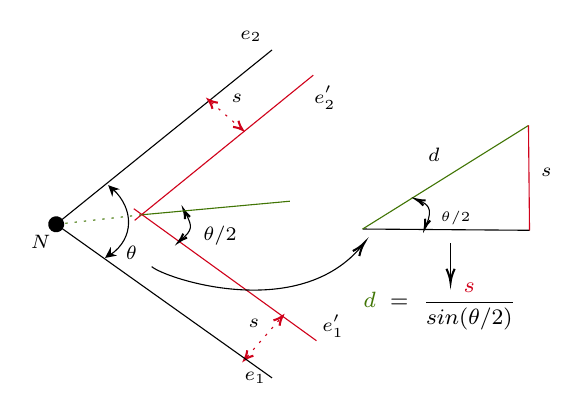
\begin{tikzpicture}[x=0.75pt,y=0.75pt,yscale=-1,xscale=1]
%uncomment if require: \path (0,300); %set diagram left start at 0, and has height of 300

%Straight Lines [id:da040119542158275845] 
\draw    (74.96,146.08) -- (178.96,62.08) ;
%Curve Lines [id:da8293026312934688] 
\draw    (101.21,160.68) .. controls (112.52,152.9) and (112.54,138.62) .. (102.31,129.15) ;
\draw [shift={(100.03,127.25)}, rotate = 44.62] [fill={rgb, 255:red, 0; green, 0; blue, 0 }  ][line width=0.08]  [draw opacity=0] (5.36,-2.57) -- (0,0) -- (5.36,2.57) -- (3.56,0) -- cycle    ;
\draw [shift={(98.5,162.3)}, rotate = 323.23] [fill={rgb, 255:red, 0; green, 0; blue, 0 }  ][line width=0.08]  [draw opacity=0] (5.36,-2.57) -- (0,0) -- (5.36,2.57) -- (3.56,0) -- cycle    ;
%Straight Lines [id:da044371428727159934] 
\draw [color={rgb, 255:red, 208; green, 2; blue, 27 }  ,draw opacity=1 ] [dash pattern={on 0.84pt off 2.51pt}]  (149.79,87.4) -- (163.27,99.25) ;
\draw [shift={(164.77,100.58)}, rotate = 221.34] [color={rgb, 255:red, 208; green, 2; blue, 27 }  ,draw opacity=1 ][line width=0.75]    (4.37,-1.96) .. controls (2.78,-0.92) and (1.32,-0.27) .. (0,0) .. controls (1.32,0.27) and (2.78,0.92) .. (4.37,1.96)   ;
\draw [shift={(148.29,86.08)}, rotate = 41.34] [color={rgb, 255:red, 208; green, 2; blue, 27 }  ,draw opacity=1 ][line width=0.75]    (4.37,-1.96) .. controls (2.78,-0.92) and (1.32,-0.27) .. (0,0) .. controls (1.32,0.27) and (2.78,0.92) .. (4.37,1.96)   ;
%Straight Lines [id:da7636321254468201] 
\draw [color={rgb, 255:red, 208; green, 2; blue, 27 }  ,draw opacity=1 ] [dash pattern={on 0.84pt off 2.51pt}]  (166.94,209.91) -- (182.69,191.85) ;
\draw [shift={(184,190.35)}, rotate = 131.09] [color={rgb, 255:red, 208; green, 2; blue, 27 }  ,draw opacity=1 ][line width=0.75]    (4.37,-1.96) .. controls (2.78,-0.92) and (1.32,-0.27) .. (0,0) .. controls (1.32,0.27) and (2.78,0.92) .. (4.37,1.96)   ;
\draw [shift={(165.63,211.41)}, rotate = 311.09] [color={rgb, 255:red, 208; green, 2; blue, 27 }  ,draw opacity=1 ][line width=0.75]    (4.37,-1.96) .. controls (2.78,-0.92) and (1.32,-0.27) .. (0,0) .. controls (1.32,0.27) and (2.78,0.92) .. (4.37,1.96)   ;
%Straight Lines [id:da4959645731484468] 
\draw [color={rgb, 255:red, 208; green, 2; blue, 27 }  ,draw opacity=1 ]   (112.37,138.58) -- (200.37,202.18) ;
%Straight Lines [id:da37518220757042164] 
\draw [color={rgb, 255:red, 208; green, 2; blue, 27 }  ,draw opacity=1 ]   (112.77,144.18) -- (198.86,74.23) ;
%Straight Lines [id:da03224684631327923] 
\draw [color={rgb, 255:red, 65; green, 117; blue, 5 }  ,draw opacity=1 ] [dash pattern={on 0.84pt off 2.51pt}]  (74.96,146.08) -- (116.52,141.47) ;
%Curve Lines [id:da6196010222690171] 
\draw    (135.54,153.21) .. controls (140.32,148.98) and (140.94,147.45) .. (137.35,140.79) ;
\draw [shift={(136.39,139.06)}, rotate = 64.81] [color={rgb, 255:red, 0; green, 0; blue, 0 }  ][line width=0.75]    (4.37,-1.32) .. controls (2.78,-0.56) and (1.32,-0.12) .. (0,0) .. controls (1.32,0.12) and (2.78,0.56) .. (4.37,1.32)   ;
\draw [shift={(133.97,154.58)}, rotate = 315.94] [color={rgb, 255:red, 0; green, 0; blue, 0 }  ][line width=0.75]    (4.37,-1.32) .. controls (2.78,-0.56) and (1.32,-0.12) .. (0,0) .. controls (1.32,0.12) and (2.78,0.56) .. (4.37,1.32)   ;
%Straight Lines [id:da6848739970418427] 
\draw    (74.96,146.08) -- (178.96,220.08) ;
\draw [shift={(74.96,146.08)}, rotate = 35.43] [color={rgb, 255:red, 0; green, 0; blue, 0 }  ][fill={rgb, 255:red, 0; green, 0; blue, 0 }  ][line width=0.75]      (0, 0) circle [x radius= 3.35, y radius= 3.35]   ;
%Straight Lines [id:da19412102153259814] 
\draw [color={rgb, 255:red, 65; green, 117; blue, 5 }  ,draw opacity=1 ]   (116.52,141.47) -- (187.52,134.97) ;
%Straight Lines [id:da08103351548467064] 
\draw    (222.62,148.36) -- (303.02,148.97) ;
%Straight Lines [id:da7746295407362944] 
\draw [color={rgb, 255:red, 65; green, 117; blue, 5 }  ,draw opacity=1 ]   (222.62,148.36) -- (302.52,98.47) ;
%Straight Lines [id:da6727152009251198] 
\draw [color={rgb, 255:red, 208; green, 2; blue, 27 }  ,draw opacity=1 ]   (302.52,98.47) -- (303.02,148.97) ;
%Curve Lines [id:da10208771376844283] 
\draw    (253.39,146.1) .. controls (256.77,138.23) and (253.6,136.34) .. (250.18,134.84) ;
\draw [shift={(248.39,134.06)}, rotate = 23.36] [color={rgb, 255:red, 0; green, 0; blue, 0 }  ][line width=0.75]    (4.37,-1.32) .. controls (2.78,-0.56) and (1.32,-0.12) .. (0,0) .. controls (1.32,0.12) and (2.78,0.56) .. (4.37,1.32)   ;
\draw [shift={(252.52,147.97)}, rotate = 288.75] [color={rgb, 255:red, 0; green, 0; blue, 0 }  ][line width=0.75]    (4.37,-1.32) .. controls (2.78,-0.56) and (1.32,-0.12) .. (0,0) .. controls (1.32,0.12) and (2.78,0.56) .. (4.37,1.32)   ;
%Curve Lines [id:da6567322872014665] 
\draw    (120.98,166.47) .. controls (127.97,172.41) and (192.16,193.54) .. (222.55,156.12) ;
\draw [shift={(223.46,154.97)}, rotate = 127.57] [color={rgb, 255:red, 0; green, 0; blue, 0 }  ][line width=0.75]    (6.56,-1.97) .. controls (4.17,-0.84) and (1.99,-0.18) .. (0,0) .. controls (1.99,0.18) and (4.17,0.84) .. (6.56,1.97)   ;
%Straight Lines [id:da8309736780448946] 
\draw    (264.97,155.1) -- (264.97,172.1) ;
\draw [shift={(264.97,174.1)}, rotate = 270] [color={rgb, 255:red, 0; green, 0; blue, 0 }  ][line width=0.75]    (6.56,-1.97) .. controls (4.17,-0.84) and (1.99,-0.18) .. (0,0) .. controls (1.99,0.18) and (4.17,0.84) .. (6.56,1.97)   ;

% Text Node
\draw (147.6,173.07) node [anchor=north west][inner sep=0.75pt]   [align=left] {$ $};
% Text Node
\draw (107.29,155.25) node [anchor=north west][inner sep=0.75pt]  [font=\scriptsize] [align=left] {$\displaystyle \theta $};
% Text Node
\draw (158.28,82.12) node [anchor=north west][inner sep=0.75pt]  [font=\scriptsize] [align=left] {$\displaystyle s$};
% Text Node
\draw (166.38,190.72) node [anchor=north west][inner sep=0.75pt]  [font=\scriptsize] [align=left] {$\displaystyle s$};
% Text Node
\draw (144.57,145.48) node [anchor=north west][inner sep=0.75pt]  [font=\scriptsize] [align=left] {$\displaystyle \theta /2$};
% Text Node
\draw (61.5,150.26) node [anchor=north west][inner sep=0.75pt]  [font=\scriptsize] [align=left] {$\displaystyle N$};
% Text Node
\draw (164.5,216.26) node [anchor=north west][inner sep=0.75pt]  [font=\scriptsize] [align=left] {$\displaystyle e_{1}$};
% Text Node
\draw (162.5,51.62) node [anchor=north west][inner sep=0.75pt]  [font=\scriptsize] [align=left] {$\displaystyle e_{2}$};
% Text Node
\draw (202,188.26) node [anchor=north west][inner sep=0.75pt]  [font=\scriptsize] [align=left] {$\displaystyle e'_{1}$};
% Text Node
\draw (198,78.26) node [anchor=north west][inner sep=0.75pt]  [font=\scriptsize] [align=left] {$\displaystyle e'_{2}$};
% Text Node
\draw (259.07,138.48) node [anchor=north west][inner sep=0.75pt]  [font=\tiny] [align=left] {$\displaystyle \theta /2$};
% Text Node
\draw (307.38,117.86) node [anchor=north west][inner sep=0.75pt]  [font=\scriptsize] [align=left] {$\displaystyle s$};
% Text Node
\draw (252.88,107.86) node [anchor=north west][inner sep=0.75pt]  [font=\scriptsize] [align=left] {$\displaystyle d$};
% Text Node
\draw (221.8,173) node [anchor=north west][inner sep=0.75pt]  [font=\footnotesize] [align=left] {$\displaystyle \textcolor[rgb]{0.25,0.46,0.02}{d} \ =\ \frac{\textcolor[rgb]{0.82,0.01,0.11}{s}}{sin( \theta /2)}$};


\end{tikzpicture}

  \caption{Geometric demonstration of the offset that polygons must have with respect to nodes in order not to intersect. Let $e_1$ and $e_2$ be two edges converging at node \textit{N}, and \textit{s} be half of the thickness. The distance, \textit{d}, will be the minimum distance that ensures that the two polygons do not intersect.}
  \label{fig:offset}
\end{minipage}%
\hspace{1cm}
\begin{minipage}{.49\textwidth}
  \centering
  \includegraphics[width=\linewidth]{imgs/step_1.pdf}
  \caption{First step. Polygons are positioned perpendicular to each of the edges at a distance that ensures they do not intersect with each other. The example uses 3-sided polygons and shows in red the normal vector of each one used in the next steps.}
  \label{fig:step_1}
\end{minipage}
\end{figure}

\subsubsection{The convex hull of the nodes}
Once all the polygons have been created, the convex hull of all the points from the polygons is generated in a node, and the node itself is calculated for each node. 
This results in a ball-shaped shell in each node. 
Subsequently, all faces of the hulls with a normal vector parallel to an edge are removed. This process is undertaken to avoid duplicated faces when creating the final mesh.
The result of this step, using the example shown above, can be seen in \cref{fig:step_2}. 

\begin{figure}[!htbp]
  \centering
  \includegraphics[width=0.4\linewidth]{imgs/step_2.pdf}
  \caption{Second step. The convex hulls on the polygon points of each of the nodes and the nodes themselves are generated. Faces with normal vectors parallel to the polygons, shown in red, are removed from the convex hulls.}
  \label{fig:step_2}
\end{figure}

\subsubsection{Convex hull of the struts}

A similar process is followed for the struts. For each strut, a convex hull containing all the polygon points at both ends of each edge is calculated. Once more, all faces with a normal vector parallel to the edge are removed from the hull.
The convex hulls obtained from the polygons shown in \cref{fig:step_1} can be seen in \cref{fig:step_3}. 

\begin{figure}[!htbp]
  \centering
  \includegraphics[width=0.4\linewidth]{imgs/step_3.pdf}
  \caption{Third step. The convex hulls of the polygon points of each of the edges are generated. The faces whose normal vectors are perpendicular to the normal vectors of the polygons are eliminated from the convex hulls.}
  \label{fig:step_3}
\end{figure}

\subsubsection{Joining the surfaces}
The final mesh is created from the union of all the surfaces resulting from the previous steps. 
As all operations entail the calculation of convex hulls, this methodology is very fast. 
Following the obtaining of the final mesh, it is possible to smooth the mesh by subdividing its edges using the Python library Trimesh.
\cref{fig:step_4} \textcolor{blue}{A} shows the surface mesh obtained from the example shown above and its subsequent smoothing, \cref{fig:step_4} \textcolor{blue}{B}. 

\begin{figure}[!htbp]
    \centering
    \begin{subfigure}[t]{0.44\textwidth}
        \includegraphics[width = \textwidth]{imgs/step_4.pdf}
        \caption{Fourth step. All the convex hulls generated during the process are joined together.}
     \end{subfigure}
     \vspace{1cm}
    \begin{subfigure}[t]{0.44\textwidth}
        \includegraphics[width =\textwidth]{imgs/step_5.pdf}
        \caption{Smoothing of the mesh obtained from the process by subdividing the faces. This process can be repeated several times to obtain a smoother surface. In each iteration, each face is divided into four. In this example, the mesh was subdivided four times. }
     \end{subfigure}
     \caption{Final step in the process where surfaces without intersections are obtained and smoothed to enhance their appearance.}
    \label{fig:step_4}
\end{figure}

\cref{fig:hart} shows an example of a surface mesh obtained from a structure generated within the same cylinder used to generate the structure in \cref{fig:mesh_1}. 
This mesh forms a single surface without intersections.
If there are any intersections, the mesh subdivision process fails, and the final mesh obtained is not smoothed and does not form a watertight shape. 
In fact, this is what happens in the vast majority of cases. 
Due to the acute angles that usually exist between the edges at the nodes, the convex envelopes that are generated are so large that they intersect with each other. 
\cref{fig:mesh_fail} shows the mesh obtained with the same structure as in \cref{fig:mesh_1}. 
Although post-processing to remove invalid offsets has eliminated the conflicting edges, not all of them can be removed due to the safety criterion that a node cannot have fewer than four neighbours, to ensure the continuity of the structure. 
Therefore, although this methodology is useful for cases where the edge density is low, it is not reliable for the vast majority of cases and was ultimately discarded.

\begin{figure}[!htbp]
  \centering
  \includegraphics[width=0.4\linewidth]{imgs/mesh_hart.png}
  \caption{Example of continuous mesh obtained using the proposed algorithm.}
  \label{fig:hart}
\end{figure}
\begin{figure}[!htbp]
  \centering
  \includegraphics[width=0.4\linewidth]{imgs/mesh_2.png}
  \caption{Mesh obtained from the structure shown in \cref{fig:mesh_1} using the proposed algorithm. The pointed appearance denotes the existence of intersections and that the mesh is not watertight.}
  \label{fig:mesh_fail}
\end{figure}

Up to this point, all the libraries used were open source, as from the outset the aim of this project was for it to be accessible to anyone, openly and free of charge, for use.
However, as no open source solution proved successful, it was decided to turn to commercial software to generate the mesh. 
Due to the limited availability of licences for this software, it was not possible to test many different programs; however, those that were available were used, and licences were requested for software specialised in mesh generation. 
Commercial software is usually more powerful than open source libraries, as the companies that own it have entire teams dedicated to improving and optimising algorithms for generating and manipulating meshes. 
Furthermore, as mentioned above, the structures used in this project cannot be generated manually, so one requirement that the software used must meet is that it has a scripting module in some programming language to automate the generation of the meshes.
Specifically, Abaqus 2023\footnote{\href{https://www.3ds.com/products/simulia/abaqus}{Abaqus} official website.} (Dassault Systèmes, France), SolidWorks 2019\footnote{\href{https://www.solidworks.com/}{SolidWorks} official website.} (Dassault Systèmes, France) and Autodesk Fusion 360 2024\footnote{\href{https://www.autodesk.com/products/fusion-360/overview}{Autodesk Fusion 360} official website.} (Autodesk, Inc., United States) software was used. 
All of them also failed to generate the mesh. 
The errors obtained were always the same: the intersections between cylinders generated degenerate elements, invalid geometries or free edges. 
Even the mesh repair modules that these programmes have were unable to fix the invalid geometries. 
Different strategies were tried to generate the mesh using various strategies to facilitate mesh generation at intersections and nodes. 
Spheres were used at the nodes to avoid complex intersections. 
Some attempts were made to create a very fine mesh at the nodes and a coarser mesh at the edges, and also, an attempt was made to voxelise the cylinders, among other things. 
However, none of these strategies was successful.

At this point, emphasis was placed on understanding why no software was capable of meshing this type of structure. 
It should be kept in mind that the reticular structures proposed in this work are very complex, as they have very high connectivity and, being stochastic structures, the angles at which the edges converge at the nodes are usually very sharp. 
Commonly used reticular structures are regular structures with low connectivity, and the edges converge at the nodes at larger angles. 
The main problem lies in the complexity of obtaining the shape of the intersections when the number of cylinders converging at a node is very high. 
There are several ways to obtain the intersections between surfaces. 
The simplest of these is to calculate the intersection of primitives (line-line, line-plane or plane-plane), but this is only useful when the entities are simple and the number is small. 
For example, the intersection of two cylinders with the same radius that converge at a point is parabolic in shape and can be parameterised using its major and minor axes. 
With three cylinders, the intersection is a composition of parabolas. 
But when the number is much higher, there is no analytical solution to represent the intersection. 
There are proposals such as the work conducted by Zou et.al.\cite{Zou2025} that obtain the intersections by decoupling all the cylinders and calculating the intersections between pairs of them until a single one is obtained.
However, they use regular structures with medium connectivity, so the intersections they obtain are mostly parabolas.
In computer graphics, Non-uniform rational basis splines (NURBS) are used to represent surfaces that are more complex than primitive geometries. 
NURBS is a mathematical model for representing curves that can be parameterised. 
In this case, which is usually the most common, the intersection between curves is obtained by solving the equations that define each of the surfaces. 
Although it may seem simple, the surface-to-surface intersection problem can only be solved for certain types of surfaces, and approximation methods are normally used to obtain the intersection \cite{Hohmeyer}. 
These algorithms are used by OpenCASD to calculate intersections. 
As intersections are often obtained by approximation, when the angles of incidence are very small, the resulting surfaces are often degenerate. 
When attempting to obtain the intersection of previously triangulated surfaces, there are algorithms such as the one proposed by Möller–Trumbore\cite{Möller01011997}, which uses rays to calculate the intersections between triangles. 
However, its accuracy depends on the accuracy of the mesh, so if there are local intersections smaller than the size of the triangles, holes are often generated.
The same problem occurs in the Separating Axis Theorem algorithm \cite{Boyd2014} used by the CGAL library to calculate intersections.   
In addition to those mentioned above, there are many other algorithms for calculating intersections between surfaces. 
Others are not fully known, which are implemented by commercial software and are not public. 
However, they are all based on the same principles and theorems. 
The structures proposed in this work are too complex for these conventional algorithms and pose a challenge for conventional programmes when it comes to generating them, which is why they fail. 

Highly connected lattice structures are rarely used in real-world applications, mainly due to the complexity of their manufacture. 
Lattice structures used in the real world, such as those found in cranes, bridges, industrial buildings, electricity pylons, etc., are very low-connectivity, regular structures that use highly slender bars to make them easier to manufacture. 
However, thanks to the development of 3D printing, the manufacture of highly connected and irregular lattice structures has become so easy that they are increasingly seen in industrial applications. 
This has led different groups to design software capable of generating this type of structure. 
To do so, they must be able to deal with very complex intersections and, above all, develop new algorithms that allow them to be modelled. 
The algorithms mentioned above are not very robust for complex cases because they start from pre-existing geometries and attempt to find the intersection between them. 
There is a set of computational geometry algorithms that does not rely on NURBS for surface representation but rather on implicit functions to define them. 
For example, to define a sphere using NURBS, an arc of a circumference must first be defined. 
This arc is expanded to a semicircle, which is used to generate a spherical half-cap, ultimately producing a sphere. 
During this process, control points are generated in each of the geometric shapes, resulting in a sphere with many control points, joined together, which define this surface. 
In contrast, in implicit design, a sphere is obtained through its implicit function, $f(x, y, z)=\sqrt{x^2+y^2+z^2}-r$.
However, the sphere is not generated until the desired radius value is defined, as these algorithms use signed distance functions (SFD) to define these super-surfaces:
$$
f(x, y, z)= \begin{cases}<0 & \text { point inside solid } \\ =0 & \text { point on the surface } \\ >0 & \text { points outside solid }\end{cases}
.
$$
With this approach, the geometry is continuous and infinite in resolution until it is sampled on a mesh. Furthermore, Boolean operations are simply operations between functions: Union: $\min\left(f_1, f_2\right)$, Intersection: $\max\left(f_1, f_2\right)$ and Difference: $\max\left(f_1,-f_2\right)$.
This avoids all the problems that CAD programmes have when calculating intersections. 
In reality, this methodology does not calculate intersections, but rather calculates the composition of all the functions, which is called a field, and then represents them using their SFD at each point. 
In this way, the solid is not stored as a NURBS but as an implicit field without intersections.
Furthermore, this methodology is much faster as it avoids generating a multitude of solids.
There are very few software programmes that use implicit modelling, and those that do exist are relatively new. 
At the time of writing, there are only two commercial solutions focused on design and manufacturing based on implicit modelling: nTop\footnote{\href{https://www.ntop.com/}{nTop} official website.} (nTopology, United States) and Materialise 3-matic\footnote{\href{https://www.materialise.com/en/industrial/software/3-matic}{Materialise 3-matic} official website.} (Materialise, Belgium). There is also the Monolith\footnote{\href{https://andy-payne-68uu.squarespace.com/}{Monolith} official website.} programme (Autodesk Inc., United States), but this is mainly based on voxelisation to generate geometries. Thanks to the fact that nTopology offers free licences of its software to students, its software was used to generate the structure's mesh. 

nTop does not have a scripting module to automate the generation of parts, but it does have functions that allow you to create reticular structures from the coordinates of the nodes of each of the edges. 
It also allows these coordinates to be imported from a CSV file. 
So, the graph produced by the structure generation module had to be converted to a CSV file containing the coordinates of each of the edges, see \cref{fig:edges}. 
Once the skeleton of the structure has been generated, the surface of the structure is converted into an implicit body from which the surface and volumetric mesh can be generated.
\cref{fig:solid} shows the final solid mesh obtained.
Two plates were manually added to the lower and upper bases to facilitate anchoring the structure to the satellite body and the thruster, respectively.
It can be seen that several pores in the upper part have been collapsed by the programme's meshing algorithm. 
This must happen because the edges in this area are very close together due to the narrowing of the structure. Despite this, the mesh has been generated and refined without any problems. 
It is worth mentioning that this software is practically new, having been commercially launched in 2019, so it is constantly being developed and its functions are being optimised and new ones added. 
Despite this, the surface and volumetric meshes were generated in a couple of hours on a personal computer. 
In addition, it allows the processing of objects to be accelerated by partially executing some operations on the GPU.


\begin{figure}[!htbp]
    \centering
    \begin{subfigure}[t]{0.3\textwidth}
        \includegraphics[width = \textwidth]{imgs/edges.png}
        \caption{Front view of the set of virtual edges of the thruster bracket structure.}
     \end{subfigure}
     \hspace{1cm}
    \begin{subfigure}[t]{0.295\textwidth}
        \includegraphics[width =\textwidth]{imgs/edges_sec.png}
        \caption{Cross-sectional isometric view of the virtual edges of the thruster bracket structure.}
     \end{subfigure}
     \caption{First step for the creation of the stochastic reticular structure created as support for the propeller. The edges imported from the graph generated by the structure generation module are shown.}
    \label{fig:edges}
\end{figure}

\begin{figure}[!htbp]
    \centering
    \begin{subfigure}[t]{0.3\textwidth}
        \includegraphics[width = \textwidth]{imgs/solid.png}
        \caption{Front view of the solid mesh of the thruster bracket structure.}
     \end{subfigure}
     \hspace{1cm}
    \begin{subfigure}[t]{0.268\textwidth}
        \includegraphics[width =\textwidth]{imgs/solid_2.png}
        \caption{Cross-sectional isometric view of the solid mesh of the thruster bracket structure.}
     \end{subfigure}
     \caption{Final solid mesh generated of the bracket thruster.}
    \label{fig:solid}
\end{figure}
\newpage
\subsection{Finite element analysis of the meshed structure}

Once the volumetric mesh of the structure has been generated, it can be exported for simulation in other software.
Specialised software was used to perform the simulations. 
An attempt was made to simulate the structure using the version of Nastran offered by Siemens\footnote{\href{https://plm.sw.siemens.com/en-US/simcenter/mechanical-simulation/nastran/}{Nastran NX} official website.} (Siemens Industry Software Inc., United States) and Abaqus 2023. 
However, it was not possible to simulate with either of them for two reasons: the meshes generated required more computational resources than were available, and the geometry had some oblique elements. 
Regarding the first problem, the meshes generated contained many elements.
For example, the surface mesh from which the solid in \cref{fig:solid} was generated originally contained 17.5 million faces and 8.7 million nodes. 
After remeshing, it was reduced to 14 million faces and 7 million nodes.
Then, a simplification of the 80\% reduced the number of elements to 2.8 million faces and 1.4 million nodes. 
This simplified mesh was used to generate the solid mesh in the image, which contains 11.5 million cells, 15.6 million edges, and 2.6 million nodes. 
The drawback of reticular structures is that they have a lot of detail. 
The nodes are areas with complex topologies, and these areas cannot be easily meshed with coarse elements. 
Therefore, the reduction of elements can only be carried out on the edges. 
However, the surface area of the nodes is similar to or greater than that of the edges as a whole. 
Thus, the reduction is limited at the inferior point. 
For this reason, reducing the size of the structure did not significantly change the number of elements. 
To simulate such large meshes, computers with large RAM or even computer clusters are required, which were not available.
Regarding the second problem encountered, as mentioned in the section above, nTop does not work with discrete meshes but implicitly models surfaces. 
However, it allows to materialise the meshes to export them.
But when generating these meshes, certain problems associated with discrete surfaces reappear. Therefore, degenerate elements may be generated that cannot be processed by traditional solvers. There are also other programmes specialised in mesh repair that can solve these elements, but none were available. 

As the traditional solvers available did not allow the simulations to be run, it was decided to use JAX-FEM\cite{xue2023jax}. 
This is a finite element library developed in Python on JAX, a Google environment designed for automatic calculation and accelerated execution on CPUs, GPUs, and TPUs. 
Unlike commercial packages such as Abaqus, which implement highly optimised solvers in C++/Fortran but are closed in nature, JAX-FEM is designed as an open, extensible and customisable framework.
Its main advantage lies in its native integration with JAX, which allows assembly and resolution calculations to be compiled using XLA (Accelerated Linear Algebra) and executed on massively parallel computing architectures, almost entirely on the GPU. 
JAX-FEM offers the possibility of implementing ‘matrix-free’ solvers, in which the global matrix is not explicitly stored and only matrix-vector products are performed. 
This strategy significantly reduces memory consumption and allows linear elasticity problems to be addressed in large-scale domains with more limited hardware.
Although JAX-FEM seemed like a good solution, due to geometric problems in the mesh, the solver could not converge when simulating the bracket structure. 
Test simulations were successfully run with other simpler structures, demonstrating JAX-FEM's potential in terms of speed and efficiency.

At this point, the only remaining option was to use nTop's simulation module. 
Although implicit modellers are very good at generating complex meshes, simulations are not their strong point. 
To analyse structures, these frameworks generate a simplified mesh of the surface and then use simplified or external solvers to perform the analysis. 
This is why simulation modules are single-purpose and limited. 
Furthermore, they do not seek to compete with conventional solvers in terms of accuracy, but rather in speed. 
Thus, the results they produce are less accurate than those obtained with a specialised solver. 
In the version used (5.30.2), the available analyses are: static compression, modal, buckling, and steady-state thermal. 
They also have a topological optimisation module and a beta version of flow analysis.
It should also be noted that due to all the problems encountered in generating the structure's mesh, the optimisation module developed using genetic algorithms, as explained above, had to be left aside because nTop does not allow the generation of lattice structures with multiple thicknesses.
Therefore, the purpose of the simulations at this point is to verify that the proposed structure can withstand the force during launch. 
It will not be possible to optimise the structure against vibrations or to perform the corresponding simulations. Even so, the vibration modes of the structure will be calculated.

Three meshes with different edge thicknesses were generated. 
The material used was Ti6Al4V ($\rho$ = 4430 $kg/m^3$, E = 113.8 $GPa$, $\nu$ = 0.34, G =42.4 $GPa$)\footnote{These represent the values used by nTop.}. 
A very conservative mass value of 5 \textit{kg}\footnote{The MR-104H 510N (115 lbf) thruster from Aerojet Rocketdyne (California, United States) was used as a reference. Its specifications can be found \href{https://www.satcatalog.com/component/mr-104h-510n/}{here}. It has also been assumed that the thruster will be anchored to a 2.6 kg rotating platform.} was assumed for the propulsion system and the adapter as a whole. 
Given that the maximum acceleration experienced during launch is \textit{13g} and nTop does not allow the use of inertial loads for simulations, a distributed load will be applied to the upper plate of the structure. 
\cref{tab:stats} shows the thickness, mass and distributed load values applied for each of the structures. 
The mass value shown only represents the mass of the structure. 
The mass of the thruster and adapter must be added to this value. 
To obtain the distributed force value, the total mass value is multiplied by \textit{13g} and divided by the area of the top plate.


\begin{table}[!htbp]
\centering
\caption{Thickness, weight, and load applied to each of the simulated meshes.}
\label{tab:stats}
\resizebox{0.8\columnwidth}{!}{%
\begin{tabular}{|c|ccc|}
\hline
\textbf{Name}   & \textbf{Thickness [$mm$]} & \textbf{Weight [$kg$]} & \textbf{Load [$kPa$]} \\ \hline
\textbf{mesh 1} & 1                         & 1.38                   & 100.4                 \\ \hline
\textbf{mesh 2} & 2                         & 3.54                   & 134.4                 \\ \hline
\textbf{mesh 2} & 3                         & 6.32                   & 178.1                 \\ \hline
\end{tabular}%
}
\end{table}

Given that nTop is software specialised in modelling rather than simulation, which is still under development, the options for representing the results obtained are limited. 
The results obtained for displacement, Von Mises stress and natural frequencies are shown below.
Despite this, it is worth mentioning that none of the simulations took more than twenty minutes to run for any of the meshes, considering that an Intel Core 13th i7-13700HX 2.1 \textit{GHz} processor, 32 \textit{GB} of RAM, and an NVIDIA GeForce RTX 4070 Laptop GPU, and that the meshes used by nTop to perform the simulations had 1.5, 1.72, and 2.66 million elements, respectively.

\subsubsection{Mesh 1}

\begin{figure}[H]
    \centering
    \begin{subfigure}[t]{0.41\textwidth}
        \includegraphics[width = \textwidth]{imgs/mesh_1_disp_1.pdf}
     \end{subfigure}
     \hspace{1cm}
    \begin{subfigure}[t]{0.32\textwidth}
        \includegraphics[width =\textwidth]{imgs/mesh_1_disp_2.pdf}
     \end{subfigure}
     \caption{Front view and cross-section of the displacement results obtained for mesh 1.}
    \label{fig:mesh_1_disp}
\end{figure}

\begin{figure}[H]
    \centering
    \begin{subfigure}[t]{0.31\textwidth}
        \includegraphics[width = \textwidth]{imgs/mesh_1_stress_1.pdf}
     \end{subfigure}
     \hspace{1cm}
    \begin{subfigure}[t]{0.58\textwidth}
        \includegraphics[width =\textwidth]{imgs/mesh_1_stress_2.pdf}
     \end{subfigure}
     \caption{Front view and cross-section of the Von Mises values obtained for mesh 1.}
    \label{fig:mesh_1_stress}
\end{figure}

\subsubsection{Mesh 2}
\begin{figure}[H]
    \centering
    \begin{subfigure}[t]{0.4\textwidth}
        \includegraphics[width = \textwidth]{imgs/mesh_2_disp_1.pdf}
     \end{subfigure}
     \hspace{1cm}
    \begin{subfigure}[t]{0.4\textwidth}
        \includegraphics[width =\textwidth]{imgs/mesh_2_disp_2.pdf}
     \end{subfigure}
     \caption{Front view and cross-section of the displacement results obtained for mesh 2.}
    \label{fig:mesh_2_disp}
\end{figure}

\begin{figure}[H]
    \centering
    \begin{subfigure}[t]{0.38\textwidth}
        \includegraphics[width = \textwidth]{imgs/mesh_2_stress_1.pdf}
     \end{subfigure}
     \hspace{1cm}
    \begin{subfigure}[t]{0.52\textwidth}
        \includegraphics[width =\textwidth]{imgs/mesh_2_stress_2.pdf}
     \end{subfigure}
     \caption{Front view and cross-section of the Von Mises values obtained for mesh 2.}
    \label{fig:mesh_2_stress}
\end{figure}

\subsubsection{Mesh 3}
\begin{figure}[H]
    \centering
    \begin{subfigure}[t]{0.4\textwidth}
        \includegraphics[width = \textwidth]{imgs/mesh_3_disp_1.pdf}
     \end{subfigure}
     \hspace{1cm}
    \begin{subfigure}[t]{0.4\textwidth}
        \includegraphics[width =\textwidth]{imgs/mesh_3_disp_2.pdf}
     \end{subfigure}
     \caption{Front view and cross-section of the displacement results obtained for mesh 3.}
    \label{fig:mesh_3_disp}
\end{figure}

\begin{figure}[H]
    \centering
    \begin{subfigure}[t]{0.38\textwidth}
        \includegraphics[width = \textwidth]{imgs/mesh_3_stress_1.pdf}
     \end{subfigure}
     \hspace{1cm}
    \begin{subfigure}[t]{0.53\textwidth}
        \includegraphics[width =\textwidth]{imgs/mesh_3_stress_2.pdf}
     \end{subfigure}
     \caption{Front view and cross-section of the Von Mises values obtained for mesh 3.}
    \label{fig:mesh_3_stress}
\end{figure}

\subsubsection{Eigenfrequencies}

\begin{table}[H]
\centering
\caption{First five natural frequencies obtained for each of the simulated meshes.}
\label{tab:freqs}
\resizebox{0.8\columnwidth}{!}{%
\begin{tabular}{c|ccccc|}
\cline{2-6}
\textbf{}                             & \textbf{$\omega_0$\;[Hz]} & \textbf{$\omega_1$\;[Hz]} & \textbf{$\omega_2$\;[Hz]} & \textbf{$\omega_3$\;[Hz]}   & \textbf{$\omega_4$\;[Hz]}   \\ \hline
\multicolumn{1}{|c|}{\textbf{Mesh 1}} & 284.3             & 342.3         & 818.5         & 1171.8 & 1211.8 \\ \hline
\multicolumn{1}{|c|}{\textbf{Mesh 2}} & 455.7             & 556.1         & 1163.4        & 1680.7 & 1867.8 \\ \hline
\multicolumn{1}{|c|}{\textbf{Mesh 3}} & 561.6             & 688.0         & 1379.3        & 2023.5 & 2226.7 \\ \hline
\end{tabular}%
}
\end{table}


The results obtained from the simulations indicate that all proposed configurations will meet the vibration and compression standards mandated by the European Space Agency. 
Regarding the compression test, the displacements obtained are minimal, and the Von Mises stresses are far below the elastic limit of the material; therefore, no deformation would be apparent in any of the cases. 
Concerning the vibration test, \cref{tab:vibration_levels} summarises the frequencies to which the part is subjected during the test. 
The most energetic frequencies are experienced in the low-frequency sinusoidal test. 
This test is performed to verify that the structure does not resonate at low frequencies. 
In this range, the displacements are large and so are the accelerations, which is useful for checking the overall rigidity. 
Therefore, the first natural frequency mode of the structure must be greater than the highest frequency used during this test, 110 \textit{Hz}. 
For safety reasons, the further away this mode is, the less likely the structure is to enter into resonance. 
The random vibration test aims to simulate the vibrations experienced during launch. 
These vibrations are less energetic as the accelerations are lower, the associated displacements are small, and the high-frequency structural modes have very low effective mass. 
Therefore, ensuring that the first natural mode exceeds 200 \textit{Hz} will be more than sufficient to guarantee passing the vibration test.
The lowest natural mode calculated by nTop is 284.3 \textit{Hz} corresponding to mesh 1, so this proposed structure would be sufficient to pass both tests. 
In view of these results, a structure with the highest possible porosity was generated to reduce the total mass further.

The maximum pore size allowed for this geometry is 250 $mm^3$. 
The algorithm is not capable of generating a structure with greater porosity while respecting the shape of the specified geometry. 
Two meshes were generated from the graph obtained: one with a thickness of 1.3 \textit{mm} and another with a thickness of 2 \textit{mm}. 
The first was generated with the minimum thickness allowed by nTop in order to generate a continuous surface. 
No thicker structures were generated, as the properties of the second mesh were greater than those of the 1 \textit{mm} thick structure shown above. 
\cref{tab:stats_2} shows the thickness, weight and distributed load for each of the two meshes.

\begin{table}[!htbp]
\centering
\caption{Thickness, weight, and load applied to each of the simulated meshes with a pore size of 250 $mm^3$}
\label{tab:stats_2}
\resizebox{0.8\columnwidth}{!}{%
\begin{tabular}{|c|ccc|}
\hline
\textbf{Name}   & \textbf{Thickness [$mm$]} & \textbf{Weight [$kg$]} & \textbf{Load [$kPa$]} \\ \hline
\textbf{Mesh 4} & 1.3                         & 1.26                   & 79.4                 \\ \hline
\textbf{Mesh 5} & 2                         & 2.31                   & 113.5                 \\ \hline
\end{tabular}%
}
\end{table}

The results obtained for displacement, stresses, and natural frequencies for the two meshes generated are shown below.

\subsubsection{Mesh 4}

\begin{figure}[H]
    \centering
    \begin{subfigure}[t]{0.41\textwidth}
        \includegraphics[width = \textwidth]{imgs/mesh_1-3_disp_1.pdf}
     \end{subfigure}
     \hspace{1cm}
    \begin{subfigure}[t]{0.41\textwidth}
        \includegraphics[width =\textwidth]{imgs/mesh_1-3_disp_2.pdf}
     \end{subfigure}
     \caption{Front view and cross-section of the displacement results obtained for the mesh of thickness 1.3 \textit{mm}.}
    \label{fig:mesh_1-3_disp}
\end{figure}

\begin{figure}[H]
    \centering
    \begin{subfigure}[t]{0.45\textwidth}
        \includegraphics[width = \textwidth]{imgs/mesh_1-3_stress_1.pdf}
     \end{subfigure}
     \hspace{1cm}
    \begin{subfigure}[t]{0.45\textwidth}
        \includegraphics[width =\textwidth]{imgs/mesh_1-3_stress_2.pdf}
     \end{subfigure}
     \caption{Front view and cross-section of the Von Mises values obtained for the mesh of thickness 1.3 \textit{mm}.}
    \label{fig:mesh_1-3_stress}
\end{figure}


\subsubsection{Mesh 5}

\begin{figure}[H]
    \centering
    \begin{subfigure}[t]{0.41\textwidth}
        \includegraphics[width = \textwidth]{imgs/mesh_2_disp_1_250.pdf}
     \end{subfigure}
     \hspace{1cm}
    \begin{subfigure}[t]{0.41\textwidth}
        \includegraphics[width =\textwidth]{imgs/mesh_2_disp_2_250.pdf}
     \end{subfigure}
     \caption{Front view and cross-section of the displacement results obtained for the mesh of thickness 2 \textit{mm}.}
    \label{fig:mesh_2_disp_250}
\end{figure}

\begin{figure}[H]
    \centering
    \begin{subfigure}[t]{0.42\textwidth}
        \includegraphics[width = \textwidth]{imgs/mesh_2_stress_1_250.pdf}
     \end{subfigure}
     \hspace{1cm}
    \begin{subfigure}[t]{0.485\textwidth}
        \includegraphics[width =\textwidth]{imgs/mesh_2_stress_2_250.pdf}
     \end{subfigure}
     \caption{Front view and cross-section of the Von Mises values obtained for the mesh of thickness 2 \textit{mm}.}
    \label{fig:mesh_2_stress_250}
\end{figure}

\subsubsection{Eigenfrequencies}

\begin{table}[H]
\centering
\caption{First five natural frequencies obtained for each of the second round meshes.}
\label{tab:freqs_2}
\resizebox{0.8\columnwidth}{!}{%
\begin{tabular}{c|ccccc|}
\cline{2-6}
\textbf{}                             & \textbf{$\omega_0$\;[Hz]} & \textbf{$\omega_1$\;[Hz]} & \textbf{$\omega_2$\;[Hz]} & \textbf{$\omega_3$\;[Hz]}   & \textbf{$\omega_4$\;[Hz]}   \\ \hline
\multicolumn{1}{|c|}{\textbf{Mesh 4}} & 272.9             & 336.7         & 813.15         & 1113.3 & 1171.5 \\ \hline
\multicolumn{1}{|c|}{\textbf{Mesh 5}} & 388.9            & 479.4         & 1052.5        & 1465.2 & 1535.2 \\ \hline
\end{tabular}%
}
\end{table}

The results obtained once again show that the proposed structures meet the structural requirements imposed. 
The minimum natural frequency obtained, 272.9 \textit{Hz}, is still above 200 \textit{Hz}, thus ensuring that the structure would not enter into resonance during the test and would withstand the excitations involved. 
With regard to the displacement and Von Mises stress field obtained, although it is true that some bars at the bottom of the structure are beginning to be stressed, the resulting stresses remain below the elastic limit of the material and, therefore, no permanent deformation would be generated. 
The maximum displacement obtained remains negligible, although it should be noted that it is mainly located in one area of the structure and is not distributed throughout the structure, as can be seen in \cref{fig:mesh_1-3_disp}. 
This shows the anisotropic nature of the structure expected from a stochastic structure. 
As it is not possible to generate a structure with a lower weight due to the limitations of the algorithm for generating the skeleton and the mesher for generating the mesh, it can be concluded that Mesh 4, generated with a pore size of 250 $mm^3$, would be the best candidate for use as a satellite thruster bracket, in view of the simulated results. 
The following section shows how one of the proposed structures was manufactured.
\end{document}